\documentclass[a4paper, 12pt]{article}
% math symbols
\usepackage{amssymb}
\usepackage{amsmath}
\usepackage{mathrsfs}
\usepackage{physsummer}


\usepackage{enumitem}
\usepackage[margin = 2cm]{geometry}

\tolerance = 1000
\emergencystretch = 0.74cm



\pagestyle{empty}
\parindent = 0mm

\begin{document}

\begin{center}
  \Large{\textbf{Городской центр физического образования, 10 класс.}\\
  \textit{Серия 18, 16 февраля 2015.}}
\end{center}

\begin{center}
  \large\textbf{ Начнём вспоминать потенциал. }
\end{center}

\large

\task{ Два шарика с зарядами $q_1$ и $q_2$ имели вначале одинаковые по
  модулю и направлению скорости. После того как на некоторое время
  было включено однородное электрическое поле, направление скорости
  1-го шарика повернулось на $60^{\circ}$, а модуль скорости
  уменьшился вдвое. Направление скорости 2-го шарика повернулось на
  $90^{\circ}$.Во сколько раз изменилась скорость 2-го шарика?
  Определите модуль отношения заряда к массе для 2-го шарика, если для
  1-го он равен Электростатическим взаимодействием шариков пренебречь.
}

\task{ Пять из шести сторон правильного многоугольника образованы
  одинаковыми диэлектрическими равномерно заряженными палочками, а на
  месте шестой стороны ничего нет. При этом в точке \textbf{O},
  находящейся в центре шестиугольника, потенциал данной системы
  зарядов равен $\varphi_0$, а напряжённость электрического поля равна
  $E_0$. Найдите, какими станут потенциал $\varphi$ и напряженность
  электрического поля $E$ в точке \textbf{O}, если убрать одну из
  заряженных палочек. }

\task{ Проводящий шар радиусом $R=1$ м заряжен до потенциала
  $\varphi_1=1000$ В. Шара касаются, прикладывая плашмя к его
  поверхности тонкий незаряженный проводящий диск радиусом $r=1$ см,
  укреплённый на изолирующей рукоятке. Затем диск уносят на большое
  расстояние и разряжают. Сколько раз нужно таким образом коснуться
  шара, чтобы его потенциал стал равен $\varphi_2=999$ В? }

\taskpic[4.5cm]{ Три концентрические металлические сферы, радиусы которых
  связаны соотношением $r_1 < r_2 < r_3$, имеют заряд $q_1,q_2,q_3$
  соответственно. Найдите потенциал поля в некоторой точке \textbf{A},
  расположенной между первой и второй сферами на расстоянии $r$ от
  центра сфер, в следующих случаях: а) ключи \textbf{K1} и \textbf{K2}
  разомкнуты; б) после замыкания ключа \textbf{K1}; в) после замыкания
  ключа \textbf{K2} при замкнутом ключе \textbf{K1}. }
{
  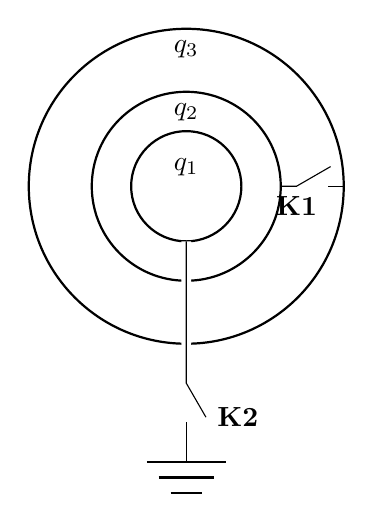
\begin{tikzpicture}
    \draw[thick] (0,0) circle (0.7cm) node[above] {$q_1$};
    \draw[thick] (0,0) circle (1.2cm) node[above=0.7cm] {$q_2$}; 
    \draw[thick] (0,0) circle (2cm) node[above=1.5cm] {$q_3$};
    \draw[draw=white,double=black,double distance=\pgflinewidth,ultra
    thick] (0,-0.7) -- ++(down:1.8cm) -- ++(300:0.5cm) node[right]
    {\textbf{K2}};
    \draw (0,-3) -- ++(down:0.5cm);
    \draw[thick] (-0.5,-3.5) -- ++(1,0);
    \draw[thick] (-0.35,-3.7) -- ++(0.7,0); 
    \draw[thick] (-0.2,-3.9) -- ++(0.4,0);
    \draw (1.2,0) -- ++(0.2,0) node[below] {\textbf{K1}} --
    ++(30:0.5cm); 
    \draw (2,0) -- ++(-0.2,0); 
  \end{tikzpicture}
}
%ru-1996-10

\end{document}


%%% Local Variables: 
%%% mode: latex
%%% TeX-engine:xetex
%%% TeX-PDF-mode: t
%%% End:
